\documentclass[10pt,twocolumn]{article} 
\usepackage{simpleConference}
\usepackage{fancyhdr}
\usepackage{amsmath,amsfonts,amssymb,graphicx}
\usepackage{subfigure}   % 使用子图形
\usepackage{indentfirst} % 中文段落首行缩进
\usepackage{bm}          % 公式中的粗体字符(用命令\boldsymbol)
\usepackage{indentfirst} % 中文首段缩进
\usepackage{abstract}    % 2栏文档,一栏摘要及关键字宏包
\usepackage{amsthm}      % 使用定理
\usepackage{booktabs}    % 使用表格
\usepackage{siunitx}
\usepackage{tikz}
\usepackage{enumitem}
\usepackage{titlesec}
\usepackage{times}
\usepackage{wasysym}
\usepackage{pifont}
\usepackage{ccaption}
\usepackage{float}
\usepackage{calc}
\usetikzlibrary{calc}
\usetikzlibrary{circuits.ee.IEC}
% 在导言区添加 circuitikz 包
\usepackage{circuitikz}
\usepackage{environ}
\usepackage{lmodern}
\usepackage{anyfontsize}
\usepackage{hyperref}
\usepackage{tabu}
\usepackage{tabularx}
\usepackage{multirow}
\usepackage{multicol}
\usepackage{longtable}
\usepackage{makecell}
\usepackage{graphicx}
\usepackage{amssymb}
\usepackage{ragged2e}
\usepackage{url,hyperref}

\newcommand*{\effXsecDPS}{\sigma_{\text{eff,DPS}}}
\newcommand*{\effXsecTPS}{\sigma_{\text{eff,TPS}}}
\newcommand*{\GeV}{~\text{GeV}}
\newcommand*{\GeVc}{~\text{GeV/c}}
\newcommand*{\GeVcs}{~\text{GeV/c}^2}

\renewcommand{\arraystretch}{1.2}

\begin{document}

\title{Search for Simultaneous Production of Double $J/\psi$ and $\Upsilon$ Mesons,\\Double $J/\psi$ and $\phi$ Mesons, or $J/\psi$, $\Upsilon$ and $\phi$ Mesons in Proton-Proton\\ Collisions at $\sqrt{s} = 13.6 ~ \mathrm{TeV}$ at the CMS Experiment}

\author{Chi Wang \\
\\
Topics on Frontiers of Cross-Sciences Course Report \\
Zhili College, Tsinghua University, China \\
\today
\\
\\
chi.w@cern.ch  \\
}

\maketitle
\thispagestyle{empty}

\begin{abstract}
The material in this template is an edited \& \LaTeX\--ified version of the recommendations here: \url{http://cs.stanford.edu/people/widom/paper-writing.html} The objective would be to help us writers, stay on topic and focused for each section of a report.

For the abstract state the problem, your approach and solution, and the main contributions of the paper. Include little if any background and motivation. Be factual but comprehensive. The material in the abstract should not be repeated later word for word in the paper. 
\end{abstract}


\section{Introduction}

\subsection{Multi-Parton Scattering in Proton-Proton Collisions}

Proton consists of three quarks, two up-type and one down-type, and gluons, which hold together the three valence quarks, as well as of a ‘sea’ of virtual quark–antiquark pairs. All these components are referred to as ‘partons’, with point-like behaviour in deep inelastic scatterings.\cite{}

In the standard picture of proton–proton (pp) collisions, typically only a few partons undergo a hard scattering with one another, with the remainders of each proton only slightly disturbed in the process. As the collision energy increases, the densities of gluons and sea quarks probed inside each proton grow rapidly. Thus, at higher collision energies, it becomes more likely for more than one pair of partons undergo a hard scattering in a single pp collision, leading to the simultaneous and independent production of two or more particles with transverse momentum ($p_T$) and/or mass ($m$) above a few giga-electronvolts. Such processes are collectively referred to as multi-parton scattering (MPS).

MPS processes offer an important probe into the complicated inner structure of the proton and its evolution with energy.\cite{DIEHL_MPI}\cite{BLOK_MPS} Many of these features, for example, the parton density profile in the plane transverse to the colliding beams, as well as the various correlations (in position, momentum, flavour, colour, spin and so on) between individual partons, are very difficult to calculate theoretically, since , and can only be mapped out through experimental studies of MPS in different systems and for different numbers $n$ of simultaneous scatterings \cite{MPI_LHC}.

In addition to providing an insight into proton structure, MPS studies also contributes to background subtraction in future searches for rare standard model and beyond-standard model resonances, especially at future hadron colliders, where the MPS contribution to the backgound becomes more significant due to higher centre-of-mass energy.\cite{DdE_TPS}\cite{YJZ_TRI_JPSI}

\subsection{The "Pocket Formula" and $\sigma_{\text{eff,NPS}}$}

Under the most simple assumption that the individual sub-scatterings are independent, one may consider the probability for the multiple production of particles with a high transverse momentum proportional to the product of the probabilities for each individual sub-scattering. This relation is more commonly expressed in terms of cross sections as the "pocket formula" shown below, for an arbitrary number $n$ of sub-scatterings:

\begin{equation}
\begin{aligned}
    \label{eqn:nps_pocket}
    &\sigma^{pp\to\psi_1+\psi_2+\cdots+\psi_n+X}_{\text{NPS}} \\&=
    \left(\frac {\mathfrak{m}}{n!}\right) \frac{\sigma_{\text{SPS}}^{pp\to \psi_1+X}\sigma_{\text{SPS}}^{pp\to \psi_2+X}\cdots\sigma_{\text{SPS}}^{pp\to \psi_n+X}}{(\sigma_{\text{eff,NPS}})^{n-1}}
\end{aligned}
\end{equation}

In the "pocket formula" (eqn. \ref{eqn:nps_pocket}), the effective cross section $\sigma_{\text{eff,NPS}}$ is only determined by the transverse parton density overlap, and the combinatorial factor $\mathfrak{m}$ is used to remove the duplicate counting from same-type particle final states.

Double parton scattering (DPS) processes are the most trivial MPS processes and the first observed. The first observation of DPS processes was made by the AFS collaboration on the Intersecting Storage Ring (ISR) at CERN\cite{ISR_DPS}. Since then, a variety of DPS processes have been studied on high-energy hadron colliders such as the Tevatron and the Large Hadron Collider (LHC).

In DPS processes, the "pocket formula" (eqn. \ref{eqn:nps_pocket}) can be more specifically written with the expression below:

\begin{equation}
\begin{aligned}
    \label{eqn:dps_pocket}
    \sigma^{pp\to\psi_1+\psi_2+X}_{\text{DPS}}=
    \left(\frac {\mathfrak{m}}{2!}\right) \frac{\sigma_{\text{SPS}}^{pp\to \psi_1+X}\sigma_{\text{SPS}}^{pp\to \psi_2+X}}{\effXsecDPS}
\end{aligned}
\end{equation}

From the proton forms adopted by event generators like Pythia8 and Herwig++, it is expected that the $\sigma_\text{eff,DPS}$ would fall in the range of $20 \to 30~\mathrm{mb}$ and would not depend on the final state studies. However, as summarized in figure \ref{fig:sigma-eff-dps-summary}, $\sigma_\text{eff,DPS}$ results obtained from experiments have been much lower, with $\sigma_\text{eff,DPS}\approx 10-20~\text{mb}$ from final states containing jets and/or electroweak bosons\cite{ATLAS_4JET_7TEV}\cite{ATLAS_WJetJet_7TEV}\cite{ATLAS_Z_JPSI}\cite{CDF_4JET}\cite{CMS_4JET_13TEV}\cite{CMS_WJETJET_7TEV}\cite{CMS_WW_DPS_8TEV_LIM}\cite{CMS_WW_DPS_13TEV_FOUND}, and even lower values of $\sigma_\text{eff,DPS}\approx 3-10~\text{mb}$ extracted from processes where two heavy quarkonia like $J/\psi$ and $\Upsilon$ are produced\cite{ATLAS_JPSIJPSI_8TEV}\cite{ATLAS_JPSI_PSI2S_7_8_TEV_COMBINED}\cite{CMS_INCL_JPSIJPSI_7TEV}\cite{ CMS_JPSIPSI2S_7TEV}\cite{CMS_JPSIPSI2S_DIFF_7TEV}\cite{CMS_YY_8TEV}\cite{CMS_YY_XSEC}.

\begin{figure}
    \centering
    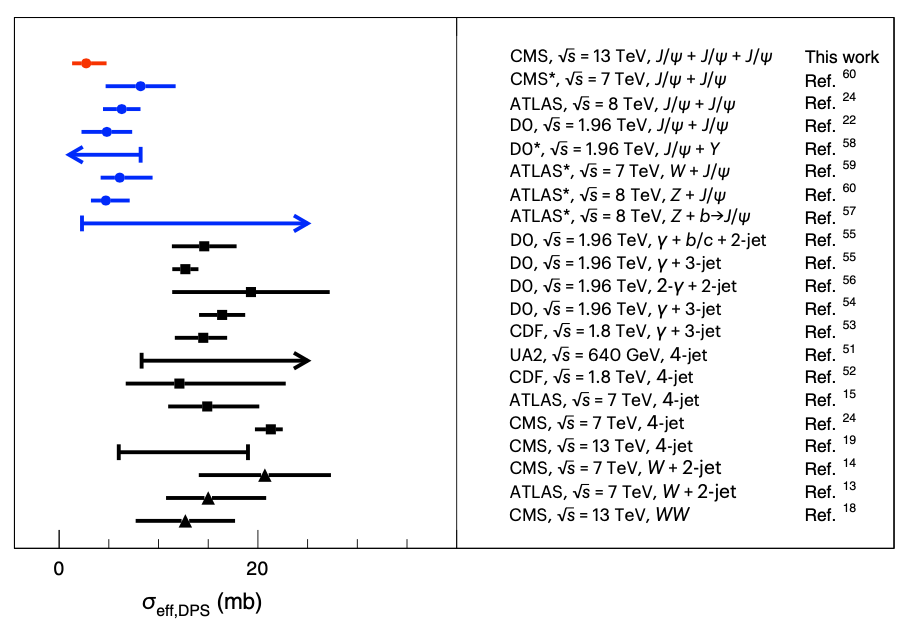
\includegraphics[width=1.0\linewidth]{images/sigma_eff_DPS_summary.png}
    \caption{Summary of current $\effXsecDPS$ measurement results in various final states\cite{CMS_TRI_JPSI}}
    \label{fig:sigma-eff-dps-summary}
\end{figure}

Disagreement in $\effXsecDPS$ obtained in different methods has been interpreted as from the difference in the dominant parton species probed through such processes \cite{MPI_at_LHC}, yet in some cases it could also be explained by inadequate SPS component subtraction. Such results calls for independent probes into the proton structure, for instance, triple parton scattering (TPS) processes.

\subsection{Triple Parton Scattering (TPS) Processes}

TPS processes in high-energy proton-proton collisions has drawn much attention both in theory and experiments. In a theoretical work by D. d'Enterria and A. M. Snigirev \cite{DdE_TPS}, it was derived across numerous transverse parton density distributions that, for a DPS processes and a TPS process with similar final states, the effective cross-sections $\effXsecDPS, \effXsecTPS$ satisfy the following relationship:

\begin{equation}
    \label{eqn:dps_tps_eff_xsec}
    \effXsecTPS = \kappa \effXsecDPS \quad (\kappa = 0.82 \pm  0.11)
\end{equation}

A more specific study on TPS processes was conducted by H.-S. Shao and Y.-J. Zhang in 2019\cite{YJZ_TRI_JPSI}, in which they demonstrated the feasibility of using existing data to observe triple-$J/\psi$ hadroproduction and, using this process, to probe into TPS processes. A further work by Y.-J. Zhang demonstrated the feasibility of observing simultaneous production of $J/\psi$, $\Upsilon$ and a $\phi$ meson with $p_T > 2\GeVc$ in high-energy proton-proton collisions\cite{YJZ_MPS_REPORT}.

The triple-$J/\psi$ production in proton-proton collision was soon observed at the CMS experiment, with a DPS effective cross-section of $\effXsecDPS = 2.7^{+1.4}_{-1.0}(\text{exp})^{+1.5}_{-1.0}(\text{theo}) ~\text{mb}$, compatible with previous $\effXsecDPS$ results from di-quarkonia processes. 

Following the pioneering studies in TPS at the CMS experiment, we are motivated to search for simultaneous production of double $J/\psi$ and $\Upsilon$ mesons, double $J/\psi$ and $\phi$ mesons, or $J/\psi$, $\Upsilon$ and $\phi$ mesons in proton-proton collisions at $\sqrt{s} = 13.6 ~ \mathrm{TeV}$ at the CMS experiment. These quarkonia final states have relatively higher cross-sections when compared to jets and electroweak bosons, bringing a larger data sample.

\subsection{The Large Hadron Collider (LHC)}

The Large Hadron Collider (LHC) operated by the European Organization of Nuclear Research (CERN) is the most powerful accelerator on earth today. The LHC is able to collide beams of protons with an energy of up to 6.8 TeV, corresponding to a center-of-mass energies of up to $\sqrt{s}=13.6~\mathrm{TeV}$. Located approximately 100 meters underground across the Swiss-Franco border near Geneva , the LHC has a main storage ring with a circumference of approximately 27 kilometers, capable of accelerating more than 2800 proton bunches simultaneously, each bunch containing approximately $10^11$ protons. Protons accelerated in the LHC traverse through the storage ring in opposite directions and intersect at four interaction points to collide at a time interval of 25 nanoseconds and deliver an instantaneous luminosity up to $2.5\times 10^{34} ~\text{cm}^{-2}\cdot\text{s}^{-1}$\cite{CMS:LUMI-PUB}. 

Particle detectors located at these interaction points, namely CMS, ATLAS, ALICE and LHCb, measure the key properties of particles produced in collision with their unique detector modules, and acquire such data for further physics analysis.

One important effect from the increasing luminosity is the "pileup" effect which refers to the phenomenon that in each bunch crossing there are usually more than one hard scattering event.\cite{CMS:LUMI-PUB} In LHC Run 3, the average number of interactions in each bunch crossing reaches 60, as shown by Figure \ref{fig:CMS_PU_Run_3}. Such effect may introduce a higher combinatorial background in the analysis and require advanced analysis techniques to mitigate its effect.



\subsection{The CMS Detector}

The Compact Muon Solenoid (CMS) (shown in Figure \ref{fig:CMS-disection}) is one of the two general-purpose detectors on LHC. The detector itself measures 21 meters long and 15 meters in diameter, with a total weight of approximately 14,000 tonnes.

\begin{figure}
    \centering
    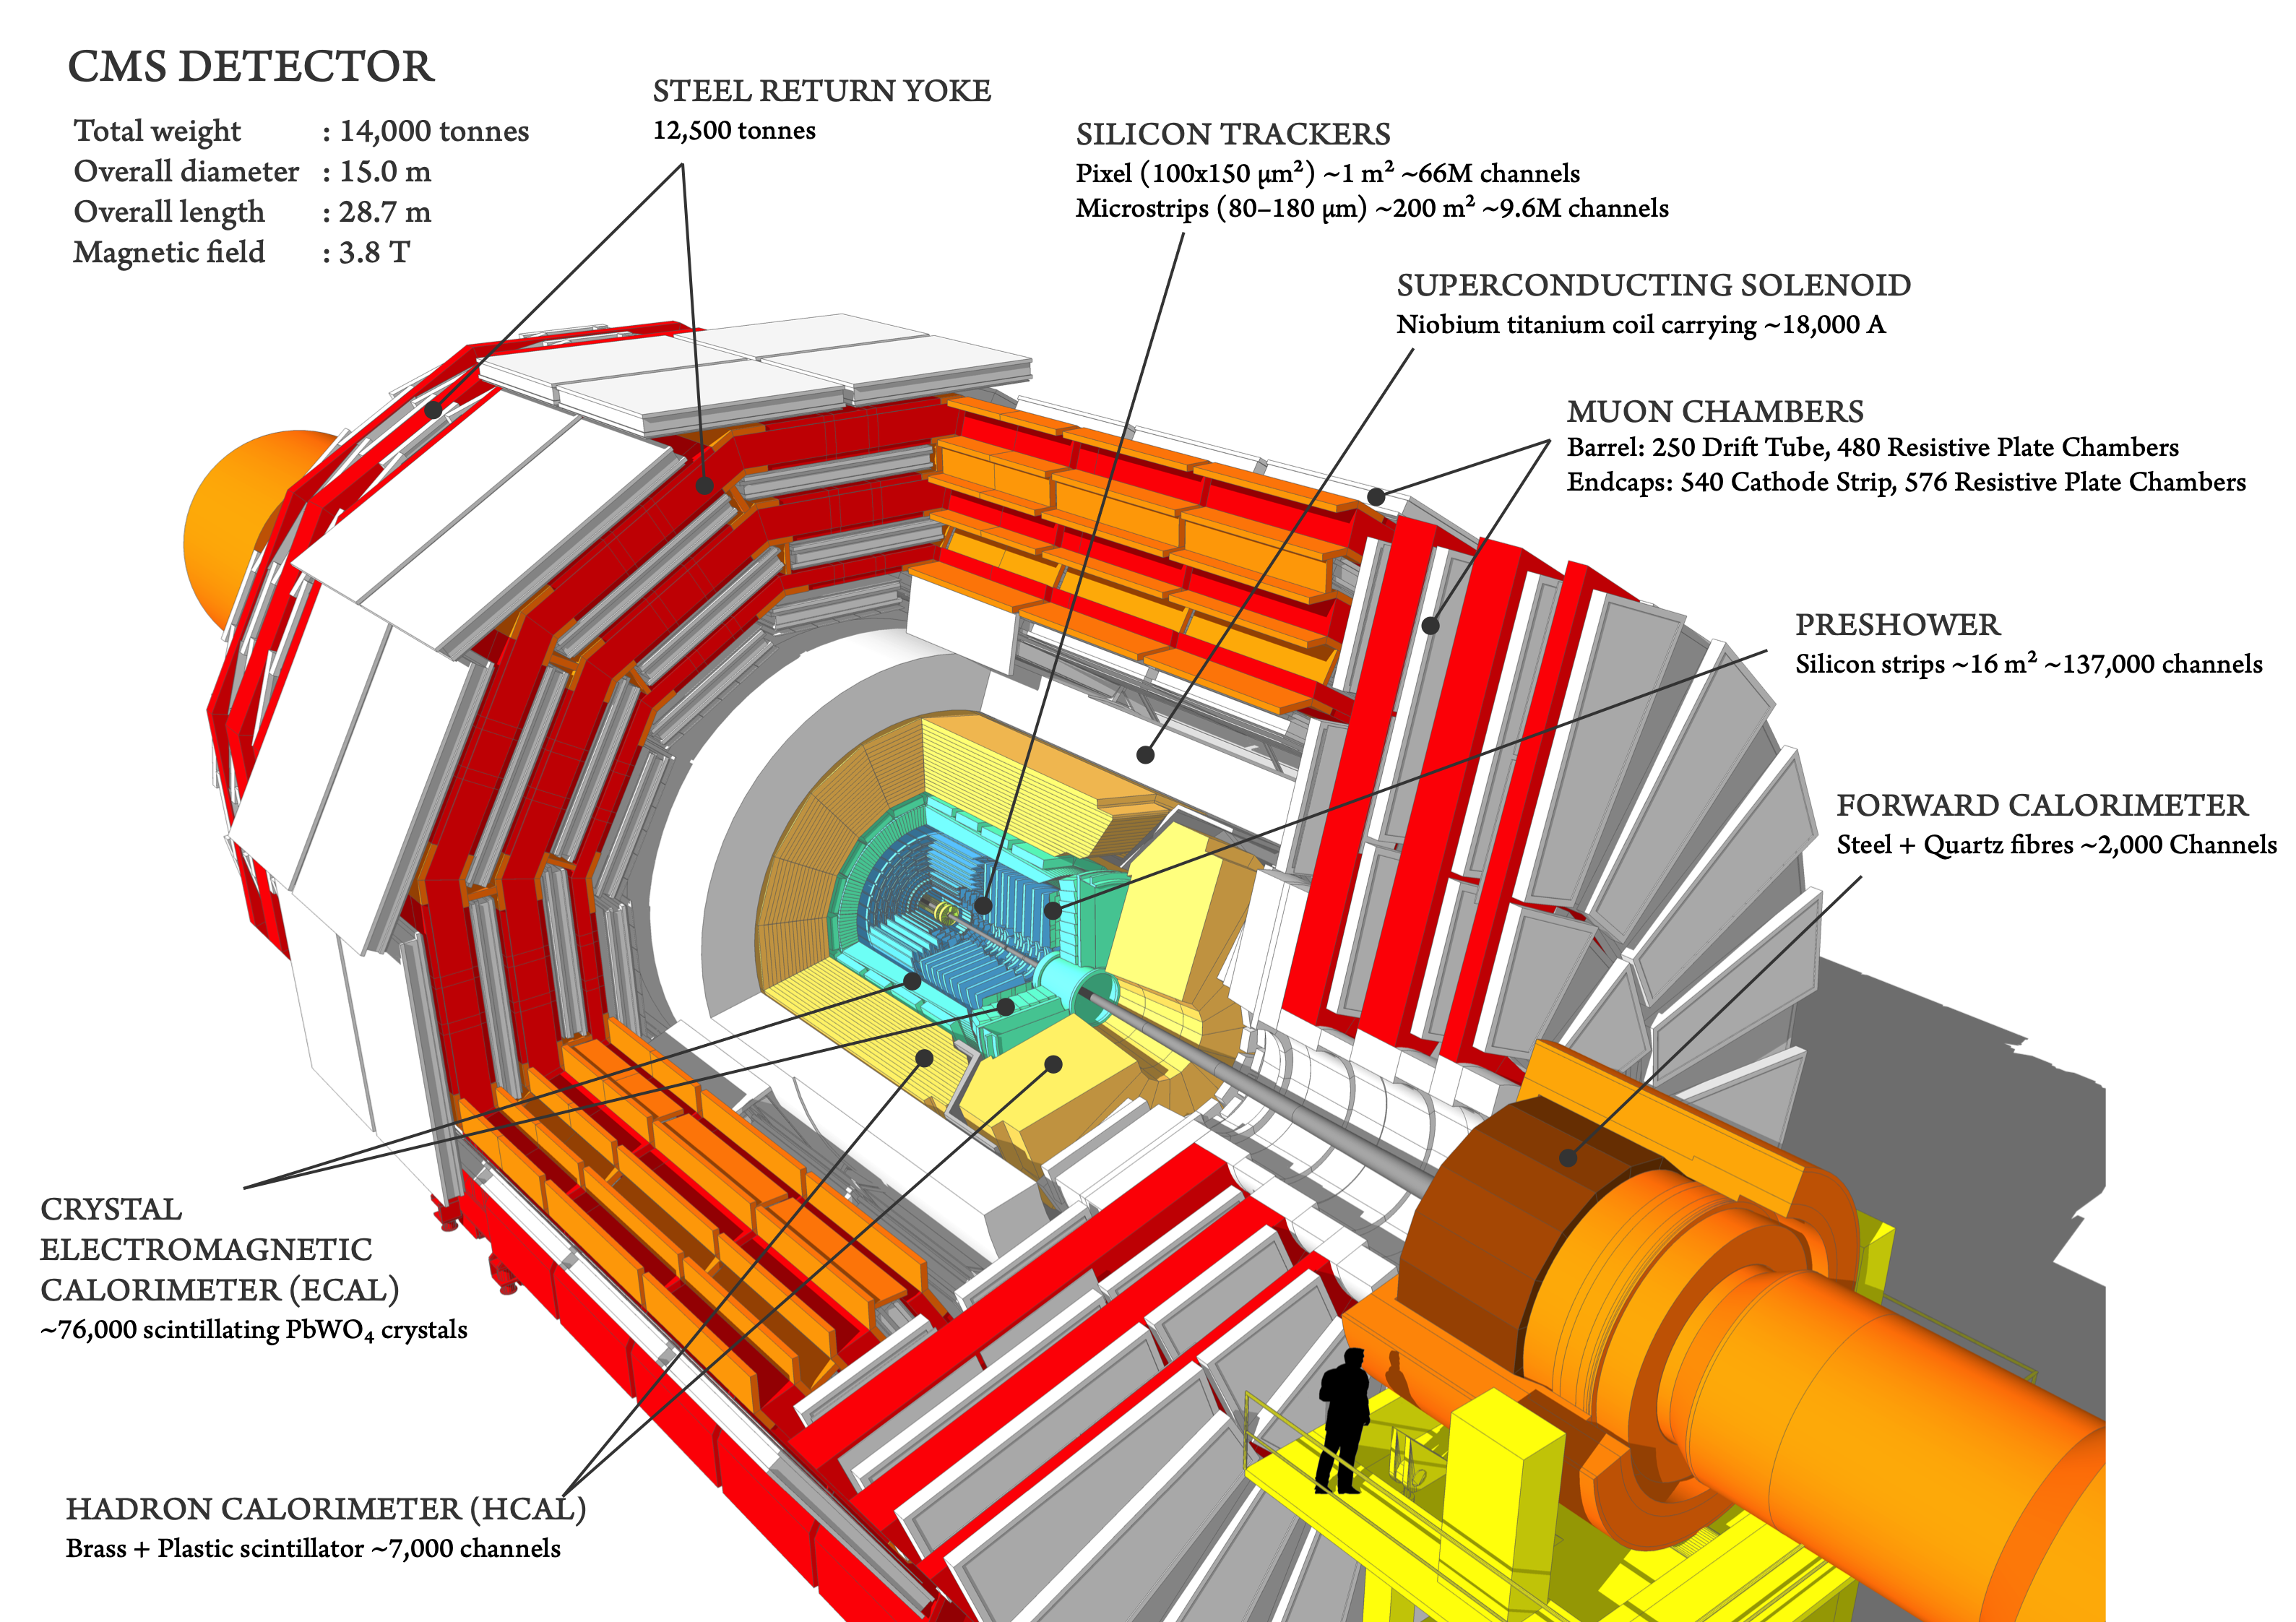
\includegraphics[width=1.0\linewidth]{images/CMS_disection_Run2.png}
    \caption{A schematic dissection of the CMS detector}
    \label{fig:CMS-disection}
\end{figure}

A defining characteristic of CMS is its powerful superconducting solenoid magnet with a inner bore of 5.9 meters and a length of 12.9 meters, capable of producing a magnetic field of 3.8 T inside its bore with a direction along the beam line, where the inner tracker and calorimeter modules are accommodated. The strong-magnetic-field design is in line with the demand for good momentum resolution within a relatively compact spectrometer.

Another distinctive advantage of CMS is its muon measurement capability, owing to its muon sub-detector module designs. With the return field of the superconducting solenoid strong enough to saturate 1.5 m of iron, the 4 muon "stations" are integrated inside the iron return yoke of the solenoid, providing a bending field of around 2 T and ensuring both robustness and full geometrical coverage. Each muon "station" consists of several layers of aluminium drift tubes (DT) in the barrel region and and cathode strip chambers (CSCs) in the endcap region, complemented by resistive plate chambers (RPCs). These detector modules work in tandem with the inner silicon tracker modules to produce a total reconstruction and identificaton efficiency of $> ~ 96\%$ and relative momentum resolution of $2\%$ for most muons and $10\%$ even for TeV muons.

\section{Dataset and Event Selection}

\subsection{Dataset}

In the present analysis, the dataset employed is the ParkingDoubleMuonLowMass collected from 2022 to 2024 certified as "muon" physics datasets, all during the LHC Run 3 period, corresponding to a center-of-mass energy of $\sqrt{s} = 13.6 ~\text{TeV}$ and an integrated luminosity of $\mathcal{L}\approx176.6~\text{fb}^{-1}$\cite{CMS:LUM-22-001}\cite{CMS:DP-LUMI-2023}\cite{CMS:LUMI-PUB}.

% \begin{figure}
%     \centering
%     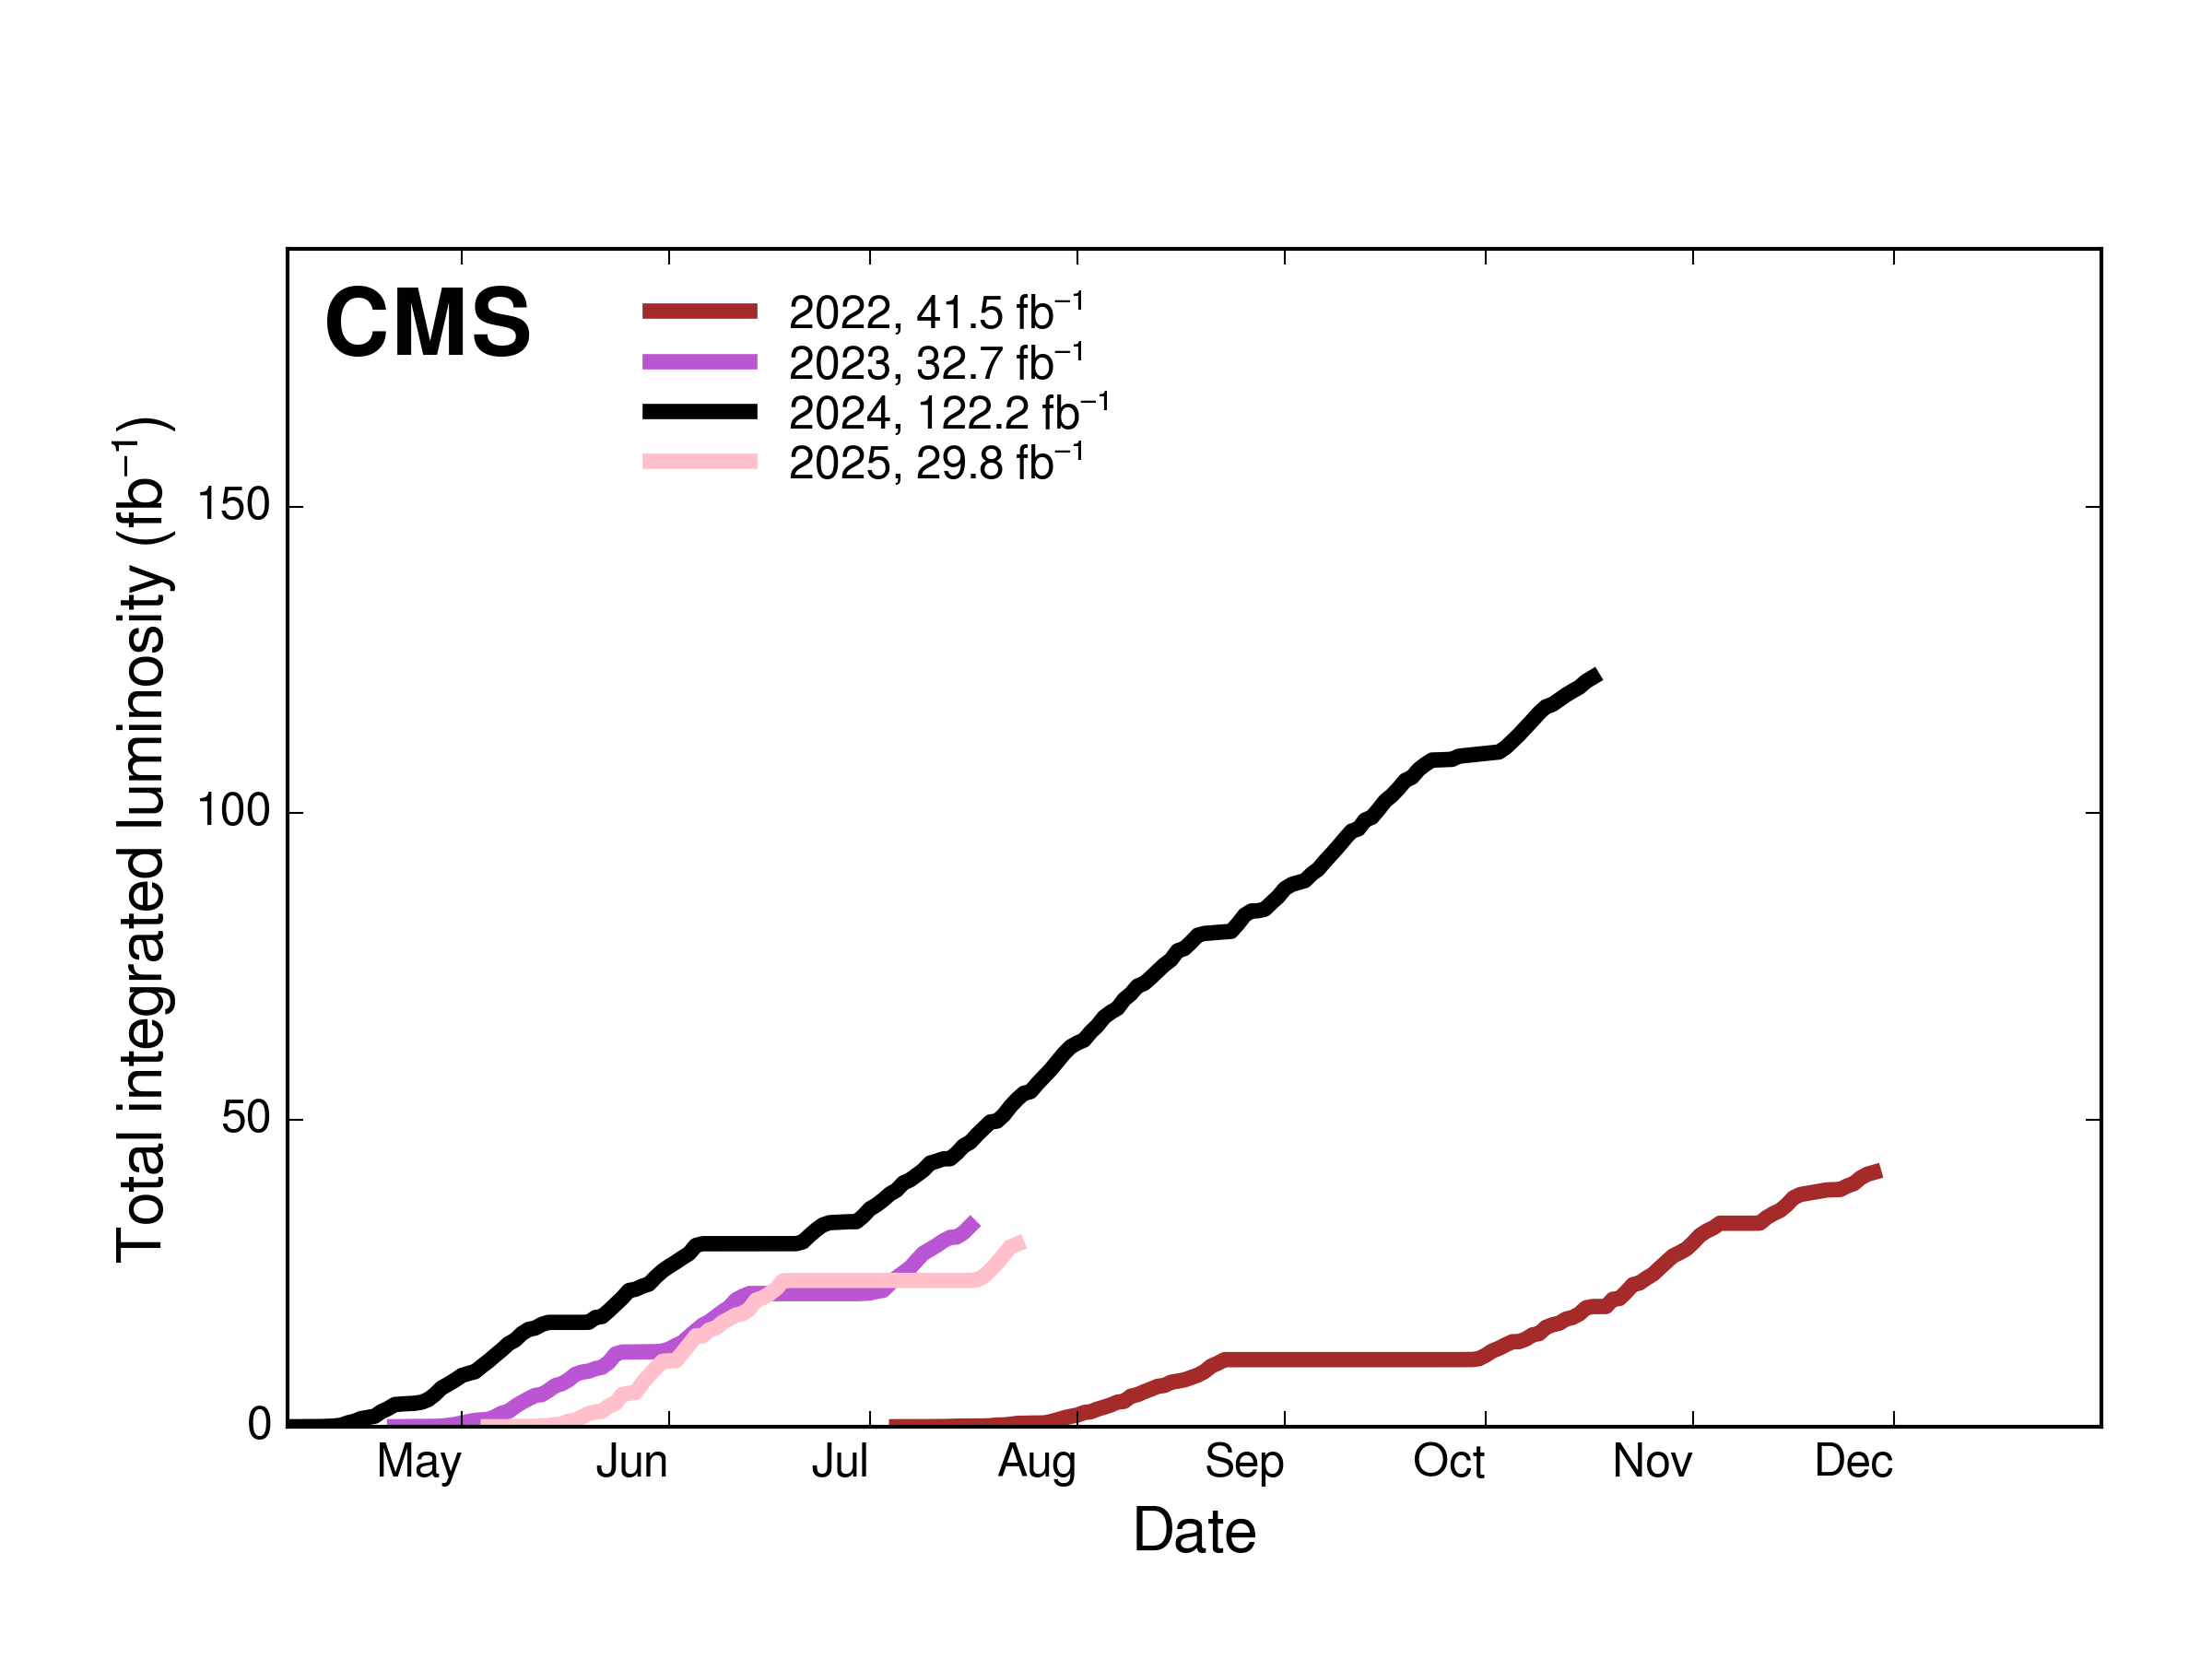
\includegraphics[width=1.0\linewidth]{images/CMS_int_lumi_Run3.png}
%     \caption{Cumulative luminosity delivered to CMS versus date during  LHC Run 3 \cite{CMS:LUMI-PUB}}
%     \label{fig:CMS_int_lumi}
% \end{figure}

\begin{table*}[h!]
    \centering
    \caption{Datasets and corresponding JSON files analyzed\\}
    \label{tab:dataset}
    \begin{tabular}{c}
    \toprule
     \multicolumn{1}{l}{\textbf{2022} - Cert\_Collisions2022\_355100\_362760\_Muon.json}\\
     ParkingDoubleMuonLowMass[0-7]/Run2022C-PromptReco-v1/MINIAOD\\
     ParkingDoubleMuonLowMass[0-7]/Run2022D-PromptReco-v1/MINIAOD\\
     ParkingDoubleMuonLowMass[0-7]/Run2022D-PromptReco-v2/MINIAOD\\
     ParkingDoubleMuonLowMass[0-7]/Run2022E-PromptReco-v1/MINIAOD\\
     ParkingDoubleMuonLowMass[0-7]/Run2022F-PromptReco-v1/MINIAOD\\
     ParkingDoubleMuonLowMass[0-7]/Run2022G-PromptReco-v1/MINIAOD\\
     \midrule
     \multicolumn{1}{l}{\textbf{2023} - Cert\_Collisions2023\_366442\_370790\_Muon.json}\\
     ParkingDoubleMuonLowMass[0-7]/Run2023C-PromptReco-v1/MINIAOD\\
     ParkingDoubleMuonLowMass[0-7]/Run2023C-PromptReco-v2/MINIAOD\\
     ParkingDoubleMuonLowMass[0-7]/Run2023C-PromptReco-v3/MINIAOD\\
     ParkingDoubleMuonLowMass[0-7]/Run2023C-PromptReco-v4/MINIAOD\\
     ParkingDoubleMuonLowMass[0-7]/Run2023D-PromptReco-v1/MINIAOD\\
     ParkingDoubleMuonLowMass[0-7]/Run2023D-PromptReco-v2/MINIAOD\\
     \midrule
     \multicolumn{1}{l}{\textbf{2024} - Cert\_Collisions2024\_378981\_386951\_Muon.json}\\
     ParkingDoubleMuonLowMass[0-7]/Run2024C-PromptReco-v1/MINIAOD\\
     ParkingDoubleMuonLowMass[0-7]/Run2024D-PromptReco-v1/MINIAOD\\
     ParkingDoubleMuonLowMass[0-7]/Run2024E-PromptReco-v1/MINIAOD\\
     ParkingDoubleMuonLowMass[0-7]/Run2024E-PromptReco-v2/MINIAOD\\
     ParkingDoubleMuonLowMass[0-7]/Run2024F-PromptReco-v1/MINIAOD\\
     ParkingDoubleMuonLowMass[0-7]/Run2024G-PromptReco-v1/MINIAOD\\
     ParkingDoubleMuonLowMass[0-7]/Run2024H-PromptReco-v1/MINIAOD\\
     ParkingDoubleMuonLowMass[0-7]/Run2024I-PromptReco-v1/MINIAOD\\
     ParkingDoubleMuonLowMass[0-7]/Run2024I-PromptReco-v2/MINIAOD\\
     \bottomrule
    \end{tabular}
\end{table*}

\subsection{Trigger Condition}

LHC collisions occur at a rate of 40 MHz, which corresponds to a data production rate of around 40 TB/s, making it impossible to store all events. The CMS experiment therfore employs a a two-tiered trigger system to preserve only events of physical importance. A hardware-based Level 1 Trigger (L1T), run on FPGAs and ASICs, reduces the event rate to 100 kHz. A software-based High Level Trigger (HLT), run on computer farms further reduces the average output rate to around 1.5 kHz.

The CMS datasets typically accept events passing any one of a certain set of trigger conditions. In our analysis, we require the events to be triggered by the HLT\_Dimuon0\_Jpsi3p5\_Muon2\_v or the HLT\_Trimuon5\_3p5\_2\_Upsilon\_Muon\_v, with the primary criteria of each trigger listed in Table \ref{tab:trigger}. The former trigger is used to extract potential $J/\psi\to\mu^+\mu^-$ processes and the latter one is used to obtain more $\Upsilon(nS)$-containing samples.

\begin{table*}[ht]
    \centering
    \caption{Primary selection criteria of the triggers employed}
    \begin{tabular}{p{0.45\textwidth}p{0.45\textwidth}}
    \toprule
    \textbf{HLT\_Dimuon0\_Jpsi3p5\_Muon2\_v}  &
    \textbf{HLT\_Trimuon5\_3p5\_2\_Upsilon\_Muon\_v} \\
    \midrule
    At least 3 muons present and satisfying: &
    At least 3 muons present and satisfying: \\
    \begin{itemize}[topsep=0pt, leftmargin=*]
        \item Transverse momentum $p_T > 2.0\GeVc$
        \item Pseudorapidity $|\eta| < 2.5$
    \end{itemize} &
    \begin{itemize}[topsep=0pt, leftmargin=*]
        \item Transverse momentum $p_T > 2.0\GeVc$
        \item Pseudorapidity $|\eta| < 2.5$
    \end{itemize}\\
    & $\mathbf{\cdot}$ At least 1 muon satisfying $p_T > 5.0 \GeVc$ \\
    \midrule
    With at least one pair of muon satisfying : &
    With at least one pair of muon satisfying : \\
    \begin{itemize}[topsep=0pt, leftmargin=*]
        \item $p_T > 3.5\GeVc$
        \item Invariant mass $m_{\mu\mu}$ satisfying $2.95\GeVcs < m_{\mu\mu} < 3.25 \GeVcs$
        \item Tracks fitted to a common vertex with probability > $0.5\%$
    \end{itemize} &
    \begin{itemize}[topsep=0pt, leftmargin=*]
        \item $p_T > 3.5\GeVc$
        \item Invariant mass $m_{\mu\mu}$ satisfying $8.5\GeVcs < m_{\mu\mu} < 11.4 \GeVcs$
        \item Tracks fitted to a common vertex with probability > $0.5\%$
    \end{itemize} \\
    \bottomrule
    \end{tabular}

    \label{tab:my_label}
\end{table*}

\subsection{Final State Particle Selection}

Given the excellent muon identification and measurement capability of the CMS detector,  we choose $J/\psi\to\mu^+\mu^-$ and $\Upsilon(nS)\to\mu^+\mu^-$ as the decay channel of these two heavy quarkonia. For $\phi$ mesons, the decay channel $\phi\to K^+K^-$ is chosen due to a relatively large branching ratio ($\approx 49\%$) \cite{PDG2020}.

In reconstruction of $\phi$ mesons, due to a relatively low identification ability for soft charged particles, all non-muon charged tracks are assumed to be $K^\pm $ and the tracks are paired only with the opposite-sign requirement.

Given that the transverse momenta of these final-state paticles typically fall in the $\text{GeV}$ region, the dominant background component for simultaneous production is the combinatorial background, with uncorrelated muons from semileptonic decay of $c$ and $b$ quarks.

To reduce background components, a further set of selection (shown in Table \ref{tab:mu_K_cuts}) is applied to the objects for event reconstruction.

\begin{table}[H]
    \centering
    \caption{Selection for final-state objects analyzed}
    \begin{tabular}{cl}
    \toprule
    Particle & Selection Criteria \\
    \midrule
    $\mu^\pm $ & Muon ID "soft" \\
              & $|\eta| < 2.4$ \\
              & $p_T > 3.5\GeVc$ for $|\eta| < 1.2$ \\
              & $p_T > 2.5\GeVc$ for $1.2 < |\eta| < 2.4$ \\
              \midrule
    Charged Tracks & High Purity \\
              & $|\eta|<2.5$ \\
              & $p_T > 2.0 \GeVc$ \\
    \bottomrule
    \end{tabular}
    \label{tab:mu_K_cuts}
\end{table}

To further reject backgrounds, we apply further individual selection for each process in the final signal extraction.

\section{Signal Extraction}

\subsection{$pp\to J/\psi+J/\psi+\phi+X$}

In extracting $pp\to J/\psi+J/\psi+\phi+X$ signals, we require further conditions shown in Table \ref{tab:cut_JpsiJpsiPhi} for the reconstructed candidate event, in which the pseudorapidity $y$ is defined by:

\begin{equation}
    y = \frac{1}{2} \ln \frac {E-p_z}{E+p_z}
\end{equation}

It is worth mentioning that the $p_T > 4.0\GeVc$ selection for $\phi$ meson is also necessary to warranty true hard-scattering processes, since $\phi(s\bar{s})$ is a light flavour meson and can be produced in large amounts in soft-QCD processes in the collision with $p_T\lesssim 2\GeVc$. A proper $p_T$ threshold can effectively remove contribution from such soft processes.

\begin{table}[]
    \centering
    \caption{Event selection for $pp\to J/\psi+J/\psi+\phi+X$ candidate events\\}
    \begin{tabular}{c p{0.66\linewidth}}
        \toprule
        \textbf{Object} & \textbf{Criteria} \\
        \midrule
        $J/\psi$ & $2.9 \GeVcs < m_{\mu\mu} < 3.3 \GeVcs$ \\
                 & $p_T > 6.0\GeVc$ \\
                 & $|y| < 2.5$ \\
                 & Opposite-sign muon pairs fitted to common vertex with $> 1\%$ probability \\
                 \midrule
        $J/\psi+J/\psi$ & Two $J/\psi$ candidates fitted to a common vertex with $> 1\%$ probability \\
        \midrule
        $\phi$ & $0.99 \GeVcs < m_{KK} < 1.07 \GeVcs$ \\
               & Opposite-sign non-muon charged tracks fitted to common vertex with $> 1\%$ probability \\
               & $p_T > 4.0\GeVc$ \\
               \midrule
        $J/\psi+J/\psi+\phi$ & Three mesons fitted to a common vertex with "valid" result \\
        \bottomrule
    \end{tabular}
    \label{tab:cut_JpsiJpsiPhi}
\end{table}

A three-dimensional maximum likelihood fit is used to extract the signal components. The $J/\psi$ signal shape is modelled with the sum of a Crystal Ball function and a Gaussian function, with all parameters left to float and background modelled by an exponential function. The $\phi$ signal shape on the di-Kaon invariant mass spectrum is taken to be a Gaussian function, also with all parameters left free to float and its combinatorial background modelled by a 4th-order polynomial. With all signal and backround components, we define further eight yield parameters.

\begin{figure}
    \centering
    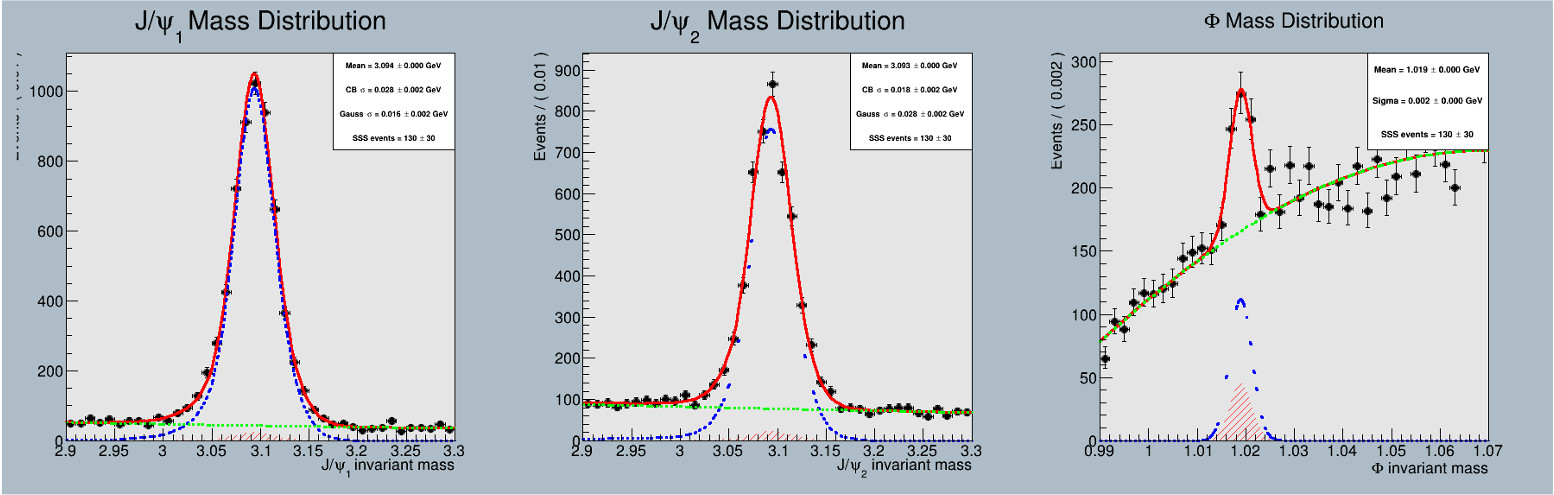
\includegraphics[width=1.0\linewidth]{images/JpsiJpsiPhi_fit.png}
    \caption{Fit result projection on individual invariant mass spectra}
    \label{fig:JpsiJpsiPhi_fit}
\end{figure}

The fit result projection is shown in Figure  \ref{fig:JpsiJpsiPhi_fit}, with $130 \pm 30$ events seen from approximately 7450 candidate events.

\begin{table}[]
    \centering
    \caption{}
    \begin{tabular}{cc}
        \toprule
        \textbf{Yield Parameter} & \textbf{Value} \\
        \midrule
        $N(J/\psi^{[1], \text{sig} },J/\psi^{[2],\text{sig} }, \phi^\text{sig})$ & $130 \pm 30$ \\
        $N(J/\psi^{[1], \text{bkg} },J/\psi^{[2],\text{sig} }, \phi^\text{sig})$ & $52 \pm 18$ \\
        $N(J/\psi^{[1], \text{sig} },J/\psi^{[2],\text{bkg} }, \phi^\text{sig})$ & $90 \pm 27$ \\
        $N(J/\psi^{[1], \text{sig} },J/\psi^{[2],\text{sig} }, \phi^\text{bkg})$ & $3476 \pm 128$ \\
        $N(J/\psi^{[1], \text{bkg} },J/\psi^{[2],\text{bkg} }, \phi^\text{sig})$ & $48 \pm 19$ \\
        $N(J/\psi^{[1], \text{bkg} },J/\psi^{[2],\text{sig} }, \phi^\text{bkg})$ & $684 \pm 55$ \\
        $N(J/\psi^{[1], \text{sig} },J/\psi^{[2],\text{bkg} }, \phi^\text{bkg})$ & $2024 \pm 120$ \\
        $N(J/\psi^{[1], \text{bkg} },J/\psi^{[2],\text{bkg} }, \phi^\text{bkg})$ & $943 \pm 54$ \\
        \bottomrule
    \end{tabular}
    \label{tab:fitres_JpsiJpsiPhi}
\end{table}

The yield parameters obtained through fitting are as listed in Table \ref{tab:fitres_JpsiJpsiPhi}. The predominant background seen from fitting is the double-$J/\psi$ with no $\phi$ mesons, and we have seen a signal significance of$4.7 \sigma$ for the simultaneous production. The efficiency and cross-section analysis are to be determined with further Monte Carlo analyses.

\subsection{$pp\to J/\psi+\Upsilon+\phi+X$}

In extracting $pp\to J/\psi+\Upsilon+\phi+X$ signals, we require further conditions shown in Table \ref{tab:cut_JpsiYPhi} for the reconstructed candidate event. Compared to the criteria required for $pp \to J/\psi+J/\psi+\phi+X$ analysis, we expect a lower cross section from the relatively low yield of $\Upsilon$ compared to $J/\psi$. We are thus motivated to lower the $p_T$ threshold for $J/\psi$ and $\phi$, to obtain more candidate events. As we look into the lower-$p_T$ regions, the combinatorial background would increase and, to compensate for this, we increased the threshold for vertex fit probabilities for $J/\psi$ and $\phi$ decay vertices to further reject backgrounds.

\begin{table}[]
    \centering
    \caption{Event selection for $pp\to J/\psi+\Upsilon+\phi+X$ candidate events\\}
    \begin{tabular}{c p{0.66\linewidth}}
        \toprule
        \textbf{Object} & \textbf{Criteria} \\
        \midrule
        $J/\psi$ & $2.9 \GeVcs < m_{\mu\mu} < 3.3 \GeVcs$ \\
                 & $p_T > 4.0\GeVc$ \\
                 & $|y| < 2.5$ \\
                 & Opposite-sign muon pairs fitted to common vertex with $> 5\%$ probability \\
                 \midrule
        $\Upsilon$ & $8.5\GeVcs < m_{\mu\mu} < 11.4 \GeVcs$ \\
                 & $p_T > 4.0\GeVc$ \\
                 & $|y| < 2.5$ \\
                 & Opposite-sign muon pairs fitted to common vertex with $> 5\%$ probability \\
                 & Reconstructed from muons passing "Tight" muon ID \\
                 \midrule
        $J/\psi+\Upsilon$ & Two candidates fitted to a common vertex with $> 1\%$ probability \\
        \midrule
        $\phi$ & $0.99 \GeVcs < m_{KK} < 1.07 \GeVcs$ \\
               & Opposite-sign non-muon charged tracks fitted to common vertex with $> 5\%$ probability \\
               & $p_T > 2.0\GeVc$ \\
               \midrule
        $J/\psi+J/\psi+\phi$ & Three mesons fitted to a common vertex with "valid" result \\
        \bottomrule
    \end{tabular}
    \label{tab:cut_JpsiYPhi}
\end{table}

A three-dimensional maximum likelihood fit is used to extract the signal components, with similar $J/\psi$ and $\phi$ signal shapes and each $\Upsilon$ resonance modelled by the sum of two CB functions, keeping only $\Upsilon(1S)$ mass and the fraction between the yields of different resonances to float.

\begin{figure}
    \centering
    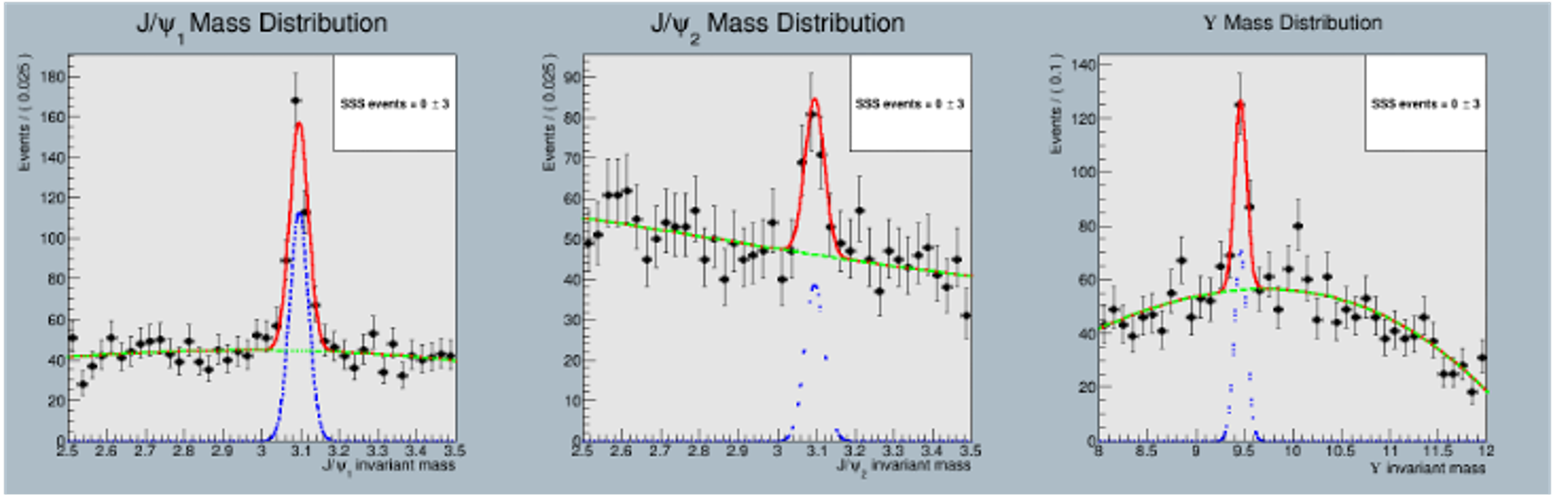
\includegraphics[width=1.0\linewidth]{images/JpsiJpsiY_fit.png}
    \caption{Fit result projection on individual invariant mass spectra}
    \label{fig:JpsiYPhi_fit}
\end{figure}

The fit result projection is shown in Figure  \ref{fig:JpsiYPhi_fit}, with $31 \pm 11$ events seen from approximately 1950 candidate events.

\begin{table}[]
    \centering
    \caption{Signal component extraction results from maximum-likelihood fit for $pp\to J/\psi+\Upsilon+\phi+X$\\}
    \begin{tabular}{cc}
        \toprule
        \textbf{Yield Parameter} & \textbf{Value} \\
        \midrule
        $N(J/\psi^{\text{sig}  },\Upsilon^{\text{sig} }, \phi^\text{sig})$ & $31 \pm 11$ \\
        $N(J/\psi^{\text{bkg}  },\Upsilon^{\text{sig} }, \phi^\text{sig})$ & $15 \pm 11$ \\
        $N(J/\psi^{\text{sig}  },\Upsilon^{\text{bkg} }, \phi^\text{sig})$ & $42 \pm 19$ \\
        $N(J/\psi^{\text{sig}  },\Upsilon^{\text{sig} }, \phi^\text{bkg})$ & $111 \pm 31$ \\
        $N(J/\psi^{\text{bkg}  },\Upsilon^{\text{bkg} }, \phi^\text{sig})$ & $43 \pm 18$ \\
        $N(J/\psi^{\text{bkg}  },\Upsilon^{\text{sig} }, \phi^\text{bkg})$ & $79 \pm 29$ \\
        $N(J/\psi^{\text{sig}  },\Upsilon^{\text{bkg} }, \phi^\text{bkg})$ & $937 \pm 55$ \\
        $N(J/\psi^{\text{bkg}  },\Upsilon^{\text{bkg} }, \phi^\text{bkg})$ & $692 \pm 51$ \\
        \bottomrule
    \end{tabular}
    \label{tab:fitres_JpsiYPhi}
\end{table}

The yield parameters obtained through fitting are as listed in Table \ref{tab:fitres_JpsiYPhi}. The predominant background seen from fitting is the single-$J/\psi$ events, and we have seen a signal significance of $2.98 \sigma$ for the simultaneous production. The efficiency and cross-section analysis are also to be determined with further Monte Carlo analyses.

\subsection{$pp\to J/\psi+J/\psi+\Upsilon+X$}

\subsubsection{Signal Extraction of $pp\to J/\psi+J/\psi+\Upsilon+X$ Process Using Maximum-Likelihood Fit}

In extracting $pp\to J/\psi+J/\psi+\Upsilon+X$ signals, we require further conditions shown in Table \ref{tab:cut_JpsiJpsiY} for the reconstructed candidate event. Compared to the $pp\to J/\psi+J/\psi+\phi+X$ process, we also expect a lower cross section from the relatively low yield of $\Upsilon$ compared to $\phi$. We are thus motivated to lower the $p_T$ threshold for $J/\psi$ again to obtain more candidate events. The threshold for vertex fit probabilities for $J/\psi$ and $\Upsilon$ decay vertices are also lowered.

\begin{table}[]
    \centering
    \caption{Event selection for $pp\to J/\psi+J/\psi+\Upsilon+X$ candidate events\\}
    \begin{tabular}{c p{0.66\linewidth}}
        \toprule
        \textbf{Object} & \textbf{Criteria} \\
        $J/\psi$ & $2.9 \GeVcs < m_{\mu\mu} < 3.3 \GeVcs$ \\
                 & $p_T > 4.0\GeVc$ \\
                 & $|y| < 2.5$ \\
                 & Opposite-sign muon pairs fitted to common vertex with $> 0.5\%$ probability \\
                 \midrule
        $\Upsilon$ & $8.5\GeVcs < m_{\mu\mu} < 11.4 \GeVcs$ \\
                 & $p_T > 3.0\GeVc$ \\
                 & $|y| < 2.5$ \\
                 & Opposite-sign muon pairs fitted to common vertex with $> 0.5\%$ probability \\
                 & Reconstructed from muons with $p_T>4.0\GeVc$ \\
                 \midrule
        $J/\psi+J/\psi$ & Two candidates fitted to a common vertex with "valid" result \\
        \midrule
        $J/\psi+J/\psi+\Upsilon$ & Three mesons fitted to a common vertex with "valid" result \\
    \end{tabular}
    \label{tab:cut_JpsiJpsiPhi}
\end{table}

A three-dimensional maximum likelihood fit is used to extract the signal components. With relatively limited statistics, the signal peaks are modelled using one Gaussian function each, with center value fixed at PDG values \cite{PDG2020} and neglecting the $\Upsilon(2S,3S)$ signals. The background is further modelled by second-order polynomials. With all signal and background components, we define further eight yield parameters.

\begin{figure}
    \centering
    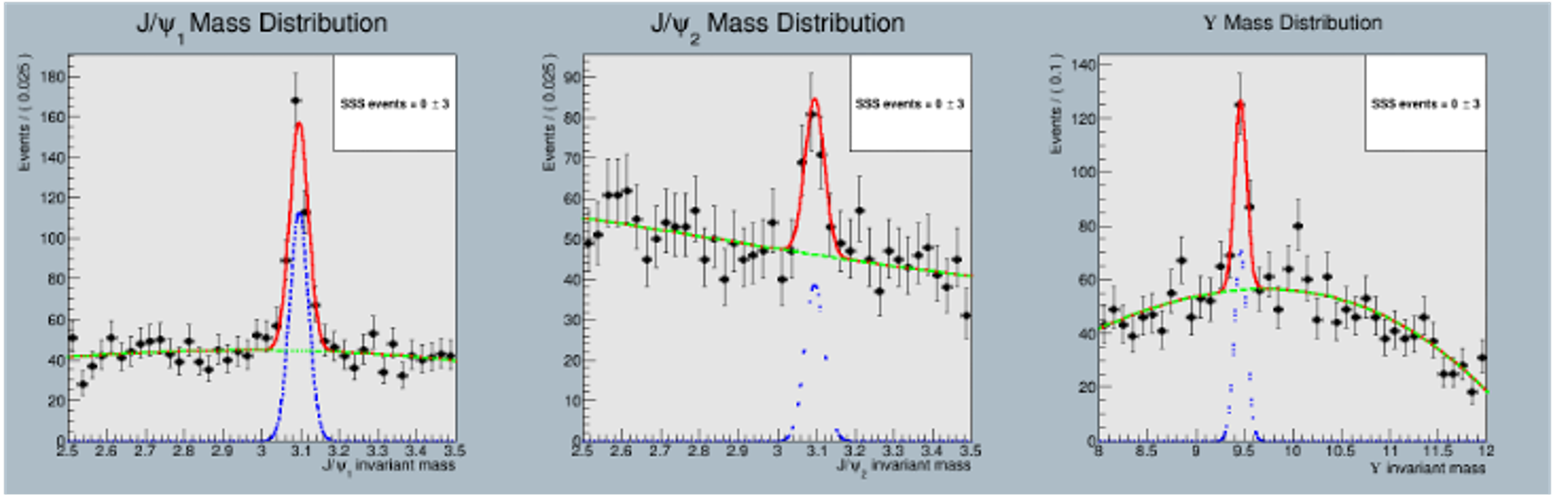
\includegraphics[width=1.0\linewidth]{images/JpsiJpsiY_fit.png}
    \caption{Fit result projection on individual invariant mass spectra}
    \label{fig:JpsiJpsiY_fit}
\end{figure}

The fit result projection is shown in Figure  \ref{fig:JpsiJpsiY_fit}, with no significant results.

\begin{table}[]
    \centering
    \caption{}
    \begin{tabular}{cc}
        \toprule
        \textbf{Yield Parameter} & \textbf{Value} \\
        \midrule
        $N(J/\psi^{[1], \text{sig} },J/\psi^{[2],\text{sig} }, \Upsilon^\text{sig})$ & $0 \pm 3$ \\
        $N(J/\psi^{[1], \text{bkg} },J/\psi^{[2],\text{sig} }, \Upsilon^\text{sig})$ & $7 \pm 7$ \\
        $N(J/\psi^{[1], \text{sig} },J/\psi^{[2],\text{bkg} }, \Upsilon^\text{sig})$ & $1 \pm 9$ \\
        $N(J/\psi^{[1], \text{sig} },J/\psi^{[2],\text{sig} }, \Upsilon^\text{bkg})$ & $9 \pm 8$ \\
        $N(J/\psi^{[1], \text{bkg} },J/\psi^{[2],\text{bkg} }, \Upsilon^\text{sig})$ & $102 \pm 19$ \\
        $N(J/\psi^{[1], \text{bkg} },J/\psi^{[2],\text{sig} }, \Upsilon^\text{bkg})$ & $80 \pm 19$ \\
        $N(J/\psi^{[1], \text{sig} },J/\psi^{[2],\text{bkg} }, \Upsilon^\text{bkg})$ & $263 \pm 25$ \\
        $N(J/\psi^{[1], \text{bkg} },J/\psi^{[2],\text{bkg} }, \Upsilon^\text{bkg})$ & $1544 \pm 48$ \\
        \bottomrule
    \end{tabular}
    \label{tab:my_label}
\end{table}

The predominant background seen from fitting is the double-$J/\psi$ with no $\Upsilon$ mesons. The low yield is believed to be due to the low cross section of the process.

\subsubsection{Estimation of $\sigma_{\text{TPS}}^{pp\to J/\psi+J/\psi+\Upsilon+X}$}

For the TPS component of the $pp\to J/\psi+J/\psi+\Upsilon+X$ process, the TPS effective cross section is taken to be $\effXsecTPS \approx 3 ~\text{mb}$ for this estimation. With SPS cross section reference values shown in Table \ref{tab:sps_xsec}, the TPS cross section is estimated to be:

\begin{equation}
    \begin{aligned}
    & \sigma_{\text{TPS}}^{pp\to J/\psi+J/\psi+\Upsilon+X} \times \mathfrak{B}_{J/\psi\to\mu\mu}^2\mathfrak{B}_{\Upsilon\to\mu\mu} \\
    & = \frac{2}{3!} \frac{\left(\sigma^{pp\to J/\psi+X}_{\text{SPS}}\right)^2\sigma^{pp\to \Upsilon+X}_{\text{SPS}}}{\effXsecTPS}\times \mathfrak{B}_{J/\psi\to\mu\mu}^2\mathfrak{B}_{\Upsilon\to\mu\mu} \\
    & = \frac{1}{3} \frac{\left(\sigma^{pp\to J/\psi+X}_{\text{SPS}}\times \mathfrak{B}_{J/\psi\to\mu\mu}\right)^2\left(\sigma^{pp\to \Upsilon+X}_{\text{SPS}}\times\mathfrak{B}_{\Upsilon\to\mu\mu}\right)}{\effXsecTPS} \\
    & \approx 0.36 ~\text{ab}
    \end{aligned} 
\end{equation}

At present statistics ($\mathcal{L} \approx 176.6 ~\text{fb}^{-1}$), we expect much less than 1 event for the TPS contribution and $\approx 1$ event with full Run 4 data ($\mathcal{L} \approx 3 ~\text{ab}^{-1}$), given present analysis strategy. Such result calls for a more efficient analysis framework.

\begin{table}[h!]
    \centering
    \caption{Caption}
    \begin{tabular}{p{0.2\linewidth} p{0.38\linewidth} p{0.35\linewidth}}
    \toprule
        Process & Fiducial Region & Estimated Cross-section \\
    \midrule
        \multirow{2}{\linewidth}{$pp\to J/\psi+X$}&
        $p_T\geq 6.0 \GeVc$ &
        \multirow{2}{\linewidth}{$\sigma(pp\to J/\psi+X) \times \mathfrak{B}_{J/\psi\to\mu\mu} \approx 80 ~\text{nb}$} \\
        & $|y| < 2.4$& \\
        \multirow{2}{\linewidth}{$pp\to \Upsilon(nS) +X$}&
        $p_T\in [10,120] \GeVc$ &
        \multirow{2}{\linewidth}{$\sigma(pp\to \Upsilon+X) \times \mathfrak{B}_{\Upsilon\to\mu\mu} \approx 1~\text{nb}$} \\
        & $|y| < 1.2$& \\
    \bottomrule
    \end{tabular}
    \label{tab:sps_xsec}
\end{table}

\section{Monte-Carlo (MC) Simulation Studies}

\subsection{Software Used for Monte Carlo Event Generation and Simulation}

HELAC-Onia 2.0 is an automated matrix element calculation tool dedicated to heavy-flavour quarkonia (such as $J/\psi$ and $\Upsilon(nS)$) studies. The matrix elements involved in heavy-flavour quarkonia production are calculated base on a NRQCD framework, giving the cross-section and dynamics characteristics in relevant processes and producing simulated events in Les Houches Event (LHE) format.

Pythia 8 is a general-purpose event generator capable of simulating processes including hard scattering, parton showering, hadronization and decay in high-energy particle collisions.

Geant 4 is a toolkit for particle-detector interaction simulation, with the capability of simulating the motion and interaction of particles in complex detector geometry and simulate the interaction between particles and detector modules in the broad energy range from eV to TeV level.

\subsection{MC Simulation Procedure Based on CMS Software (CMSSW)}

The 

\subsection{LHE-level $pp\to J/\psi+J/\psi+\Upsilon+X$ Event Simulation Studies}

\subsection{Full-chain $pp\to J/\psi+J/\psi+\Upsilon+X$ Event Simulation Results}

\section{Conclusions}

\bibliographystyle{abbrv}
\bibliography{refs}
\end{document}
